\section{Token}
Ein Token ist eine Errungenschaft, welcher ein Benutzer beim erfolgreichen Abschluss einer Quest bekommen kann. Nach Erhalt eines solchen Tokens, wird dieser im Profil angezeigt. Dadurch soll die Motivation der Benutzer gesteigert werden. 

\subsection{Variablen in der token.java}

\begin{lstlisting}[language=JAVA]
	private String title;		//Titel des Tokens
	private String description;	//Beschreibung des Tokens
	private String imagePath;	//Pfad zum Bild

	private String initPath;	//Pfad zum Packages Ordner 
	private String relPath;		//relativer Pfad zum Token
\end{lstlisting}
Title, description und imagePath, können in der zugehörigen "`.xml"' gesetzt werden. Die anderen werden beim erstmaligen Einlesen eines Tokens gesetzt und bilden die Pfade der .xml Datei. Alle hier angegebenen Variablen können mithilfe von Gettern und Settern erreicht werden.

\subsection{Odnersturktur der Tokens}
In dem Ordner mit dem Namen "`tokens"', der sich in einem Package finden lässt, befinden sich sogenannte Tokens oder auch Errungenschaften genannt. Tokens können nur innerhalb dieses bestimmten Packages verwendet werden. Somit ist es nicht möglich, sie Package-übergreifend zu benützen.
\begin{figure}[h] 
  \centering
     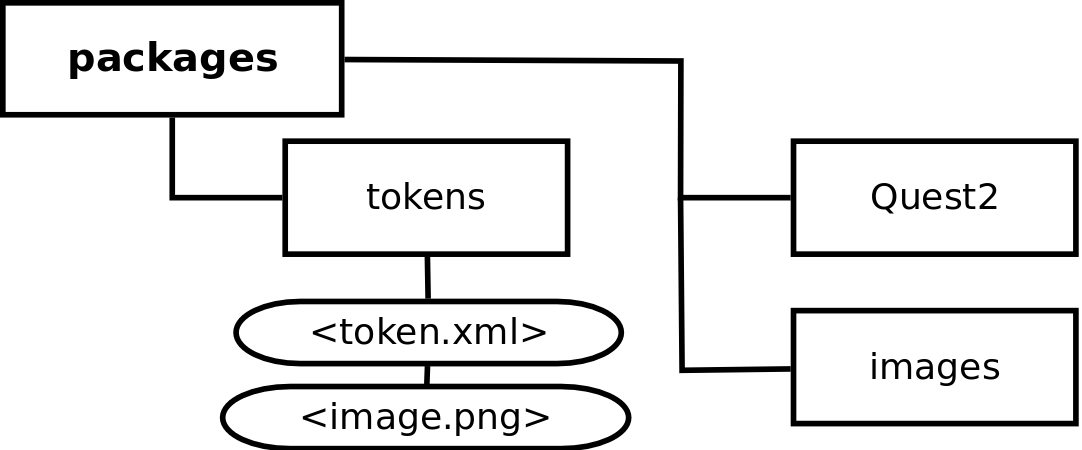
\includegraphics[width=0.8\textwidth]{./media/images/quest/token.png}
  \caption{Struktur einer Ordner}
  \label{fig:struct_token}
\end{figure}

Das Bild welches für ein Token verwendet wird, kann auch, wie in Abbildung \ref{fig:struct_token} ersichtlich, in einer gewählten Ordnerstruktur verschachtelt sein. Jedoch muss dies bei der Erstellung des "<token.xml"> berücksichtigt werden.

\subsubsection{Inhalt eines token.xml}
Der Dateiname des token.xml kann frei gewählt werden, und in der "`quest.xml"' eingetragen werden. Der Aufbau einer token.xml sieht wie folgt aus:

\begin{lstlisting}[language=XML]
<token>
	<title>Example Token</title>
	<description>Description of the Token</description>
	<imagepath>images/example.png</imagepath>
</token>
\end{lstlisting}
Hier kann ein Titel, eine Beschreibung und der Pfad zum Bild des Tokens gewählt werden. Wobei beim wählen des Bildes wichtig ist, dass hier der relative Pfad vom Ordner tokens aus, angegeben wird. Falls eine dieser Daten nicht gesetzt wurde, gilt das Token als unvollständig und kann vom Quest-System nicht weiterverarbeitet werden.